\begin{highlightblock}[Audiosignal-Synthese (10 Punkte)] \label{aufg:4}
In diesem Versuch soll die Verbindung zwischen den digitalen Signalen am PC und der \textit{realen} Welt mit Hilfe von Audiosignalen hörbar gemacht werden. Dabei lernen Sie auch ein Beispiel für ein etwas komplizierteres MATLAB-Programm kennen. Es soll ein Musikstück vertont werden. Grundlage ist die Zeit-Frequenz-Darstellung im untenstehenden Notenblatt. Horizontal ist der zeitliche Verlauf und vertikal die Frequenzlage angegeben.

\vspace{10px}

\renewcommand{\it}{}
\begin{music}
\generalsignature1 % g maj / e min (sharp on f - see circle of fifths)
\smallmusicsize
\instrumentnumber{1}
\setstaffs1{1}
\generalmeter{\meterfrac44}
\sepbarrules
\startextract
% https://ctan.joethei.xyz/macros/generic/musixtex/doc/musixdoc.pdf
% high notes: abcdefg hijklmn (starting from h is an octave higher)
% low notes:  ABCDEFG HIJKLMN 
\notes \qu d \en
\bar
\Notes \qu g \en
\notes \Dqbu gh \en 
\Notes \ql{'b} \qu{'G} \en 
\bar
\NOtes \hl{'d} \qlp{b} \en
\Notes \cl{'b} \en
\bar
\notes \ql{'c} \Dqbl dc \Dqbl bc \ql d \en 
\bar
\notes \Dqbu hg \Dqbu hi \ql{'a} \en
\setdoubleBAR
\endextract
\end{music}

Die daraus resultierende Abfolge der Töne mit den zugeordneten Zeitdauern bezogen auf ein Grundintervall ist in der Tabelle unten zusammengestellt.

\begin{center}
\begin{tabular}{*{11}{c}} % keine festen vertikalen Linien!
% Zeile 1 (Noten)
Note 
& \multicolumn{1}{c|}{d}
& g & g & a & h
& \multicolumn{1}{c|}{g} 
& d' & h
& \multicolumn{1}{c|}{h} 
& c' \\
% Zeile 2 (Dauer)
Dauer 
& \multicolumn{1}{c|}{1/4}
& 1/4 & 1/8 & 1/8 & 1/4 
& \multicolumn{1}{c|}{1/4} 
& 1/2 & 3/8 & \multicolumn{1}{c|}{1/8} 
& 1/4 \\ \hline\hline
% Zeile 3 (Noten)
Note 
& d' & c' & h 
& \multicolumn{1}{c|}{c'} & d' 
& a & g & a & h & a \\
% Zeile 4 (Dauer)
Dauer 
& 1/8 & 1/8 & 1/8
& \multicolumn{1}{c|}{1/8} 
& 1/4 & 1/8 & 1/8 & 1/8 & 1/8 & 1/4 \\
\end{tabular}
\end{center}

Der Zusammenhang zwischen den Noten und der physikalischen Signaldarstellung, d.h. die Frequenzlage, erschließt sich aus den in der Musik bekannten Beziehungen:

\begin{itemize}
\item der Kammerton \textbf{a'} entspricht einem Sinuston mit $440\mathrm{Hz}$, d.h. \textbf{a} entspricht $220\mathrm{Hz}$
\item  eine Oktave, z.B. der Übergang von \textbf{a} zu \textbf{a'}, umfasst eine Frequenzverdopplung
\item in einer Oktave gibt es $12$ Halbtonschritte
\end{itemize}

Daraus ergibt sich die Frequenzzuordnung der \textit{C-Dur}-Tonleiter ($F\cdot 220\mathrm{Hz}$)

\renewcommand{\arraystretch}{1.5} % Default value: 1

\begin{center}
\begin{tabular}{c|cccccccccccc}
Note & c & d & e & f & g & a & h/b & c' \\ \hline
Frequenzfaktor $F$ & $2^{-\tfrac{9}{12}}$ & $2^{-\tfrac{7}{12}}$ & $2^{-\tfrac{5}{12}}$ & $2^{-\tfrac{4}{12}}$ & $2^{-\tfrac{2}{12}}$ & $1$ & $2^{\tfrac{2}{12}}$ & $2^{\tfrac{3}{12}}$
\end{tabular}
\end{center}

\renewcommand{\arraystretch}{1} % Default value: 1

Mit diesen Festlegungen kann nun jeder Note ein Sinuston entsprechender Frequenz und Dauer zugeordnet werden. (Im Englischen wird für die deutsche Note \textbf{h} der Buchstabe \textbf{b} verwendet und die Tonhöhe \textbf{pitch} genannt. Durch das Vorzeichen \textbf{\#} auf der $5$. Linie von unten wird der Ton \textbf{f} um einen Halbton zum \textbf{fis} erhöht.)

\begin{itemize}
\item Machen Sie sich mit dem Programm \texttt{audiosynth.m} vertraut und starten Sie dieses.

\item Das mit dem Programm erzeugte Audiosignal klingt unnatürlich, da es nur aus jeweils ein- und ausgeschalteten Sinustönen besteht. Ein besserer Höreindruck lässt sich mit Hilfe einer Hüllkurvenbewertung erzielen. In der Audiotechnik wird hierfür oft das sogenannte ADSR-Profil (siehe Abbildung \ref{fig:adsr}) verwendet. Es besteht aus vier Geradenstücken, die die vier Phasen \textbf{Attack} (A), \textbf{Decay} (D), \textbf{Sustain} (S) und \textbf{Release} (R) repräsentieren.
\end{itemize}

\end{highlightblock}
\newpage

\begin{highlightblock}

\begin{center}
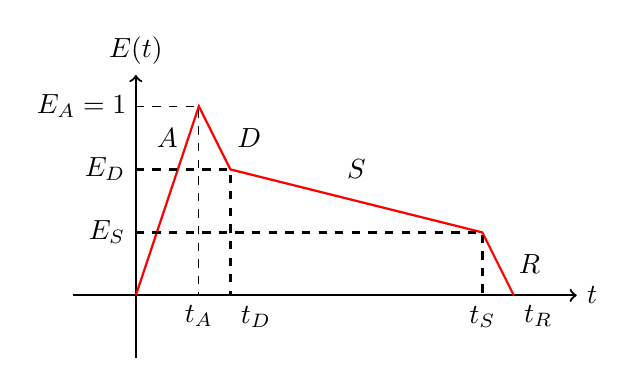
\begin{tikzpicture}[scale = 0.8]
\draw[thick, ->] (0,-1) -- (0,3.5) node[above] {$E(t)$}; 
\draw[thick, ->] (-1,0) -- (7,0) node[right] {$t$};

\draw[thick, red] (0,0) -- ++(1,3) coordinate (ea)
-- ++(0.5, -1) coordinate (ed)
-- ++(4,-1) coordinate (es)
-- ++(0.5,-1) node[below, anchor=north west, black]{$t_R$};

\draw[dashed] (ea -| 0,0) node[left]{$E_A=1$} -|
(ea |- 0,0) node[below] {$t_A$};
\draw[dashed, line width = 1pt] (ed -| 0,0) node[left]{$E_D$} -|
(ed |- 0,0) node[below, anchor=north west] {$t_D$};
\draw[dashed, line width = 1pt] (es -| 0,0) node[left]{$E_S$} -|
(es |- 0,0) node[below] {$t_S$};

\node at (0.5, 2.5) {$A$};
\node at (1.8, 2.5) {$D$};
\node at (3.5, 2) {$S$};
\node at (6.25, 0.5) {$R$};
\end{tikzpicture}
\label{fig:adsr}

Abbildung \ref{fig:adsr}: ADSR-Hüllkurve
\end{center}

\begin{enumerate}

\item[\ref{aufg:4a}] Machen Sie sich mit der Funktion \texttt{adsr\_profile.m} vertraut und modifizieren Sie in der Folge das Programm \texttt{audiosynth.m}, indem Sie die Sinustöne mit dem ADSR-Profil bewerten (mögliche Parameterwahl: $t_A = 0.15$, $t_D = 0.25$, $t_S = 0.9$, $E_D = 0.9$, $E_S = 0.7$).

\item[\ref{aufg:4b}] Erweitern Sie das Programm um die grafische Ausgabe des Musikstücks im Zeitbereich.
\item[\ref{aufg:4c}] Probieren Sie verschiedene Einstellungen für die Abtastfrequenz $f_s$, die Zeitskalierung $T$ sowie für die Parameter des ADSR-Profils aus. Kommentieren Sie Ihre Versuche kurz im Protokoll.
\item[\ref{aufg:4d}] Der Höreindruck lässt sich noch weiter verbessern, wenn Sie zusätzliche harmonische Anteile, z.B. jeweils bei der doppelten, dreifachen, etc... Frequenz, hinzunehmen. Dabei können Sie die Amplituden der Frequenzkomponenten unterschiedlich gewichten. Experimentieren Sie mit verschiedenen Einstellungen bis Sie einen zufriedenstellenden Höreindruck erhalten. Kommentieren Sie Ihre Versuche kurz im Protokoll.

\item[(e)] Erzeugen Sie eine ”WAVE”-Datei aus Ihrem finalen Musikstück. Verwenden Sie dazu den MATLAB-Befehl \m{audiowrite}. Diese Datei soll ebenfalls abgegeben werden.

\item[\ref{aufg:4f}] Mit dem Programm \texttt{kurzanalyse.m} können Sie eine Kurzzeitspektralanalyse einer Wave-Datei durchführen. Das Programm öffnet zunächst eine Audio-Datei im \texttt{wav}-Format und führt eine FFT über \textit{die gesamte Signallänge} durch. Signal und Spektrum werden dargestellt. Im zweiten Teil wird das Signal in überlappende Blöcke eingeteilt und jeder Block für sich transformiert.

\begin{enumerate}
\item Rufen Sie das Programm auf und lesen Sie die Musikdatei ein, die Sie im vorigen Punkt erzeugt haben. Wählen Sie die FFT-Länge zu $M = 4096$ und den Parameter Overlap $OL = 2$. Das FFT-Fenster wird dann jeweils um $4096/OL$ Folgenelemente weitergeschoben. Die Beträge der resultierenden Kurzzeitspektren werden zusammen als Spektrogramm angezeigt.
\item[\ref{aufg:4f2}] Rotieren Sie das Spektrogramm, so dass Sie den Frequenzinhalt über der Zeit schön beobachten können. Vergleichen Sie das Bild mit der Notenzeile. Was erkennen Sie?
\item[\ref{aufg:4f3}] Variieren Sie den Parameter der FFT-Länge (z.B. $256$, $512$, ...) und erklären Sie, was Sie in Bezug auf die Frequenz- und Zeitauflösung feststellen können.
\end{enumerate}
\end{enumerate}
\end{highlightblock}